\documentclass[border=10pt]{standalone}
\usepackage{tikz}
\usetikzlibrary{arrows.meta,positioning}

% [REVISION 2026-11] Treatments named for what they are (who sets the price); accept/reject
% stage of the price-setting-voter game shown explicitly; assignment is between sessions.

\begin{document}
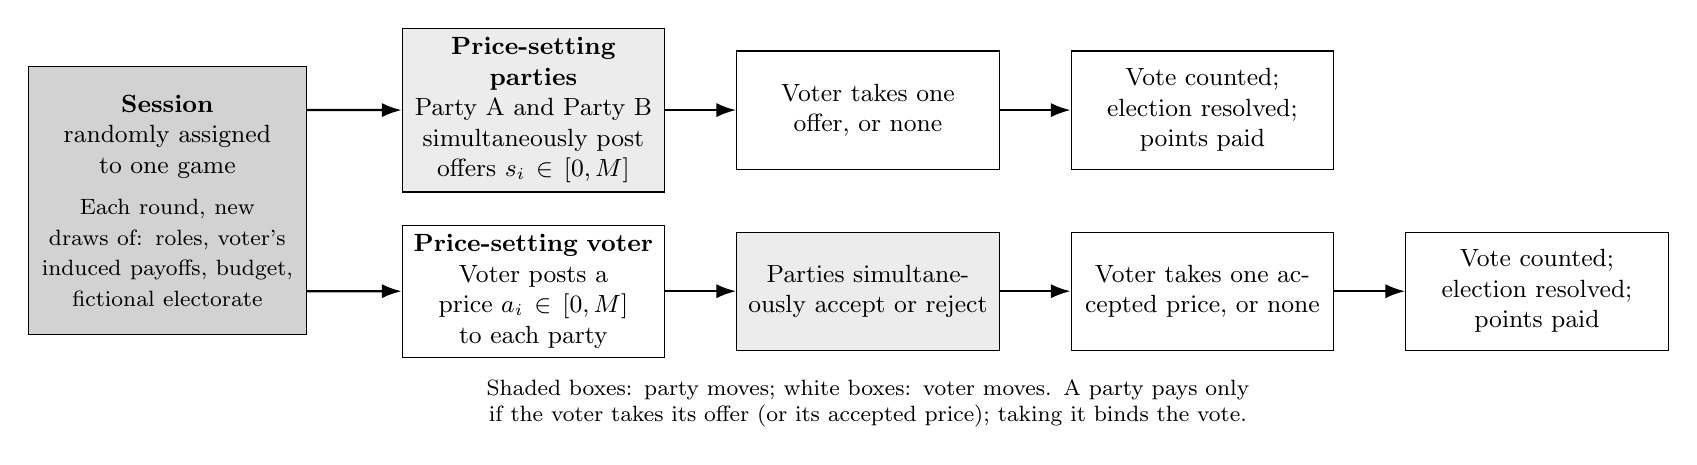
\begin{tikzpicture}[
  node distance=0.9cm,
  every node/.style={font=\small,align=center},
  box/.style={draw,minimum width=3.3cm,minimum height=1.5cm,text width=3.1cm},
  party/.style={box,fill=gray!15},
  voter/.style={box,fill=white},
  arr/.style={-{Latex[length=2.5mm,width=1.8mm]},line width=0.8pt}
]

\node[box,fill=gray!35,text width=3.3cm,minimum height=3.4cm] (RA) {
  \textbf{Session}\\randomly assigned\\to one game\\[4pt]
  {\footnotesize Each round, new draws of: roles, voter's induced payoffs, budget, fictional electorate}
};

% Price-setting parties
\node[party,right=1.2cm of RA,yshift=1.15cm] (B1) {\textbf{Price-setting parties}\\Party A and Party B simultaneously post offers $s_i\in[0,M]$};
\node[voter,right=of B1] (B2) {Voter takes one offer, or none};
\node[voter,right=of B2] (B3) {Vote counted; election resolved; points paid};
\draw[arr] (B1) -- (B2); \draw[arr] (B2) -- (B3);

% Price-setting voter
\node[voter,right=1.2cm of RA,yshift=-1.15cm] (S1) {\textbf{Price-setting voter}\\Voter posts a price $a_i\in[0,M]$ to each party};
\node[party,right=of S1] (S2) {Parties simultaneously accept or reject};
\node[voter,right=of S2] (S3) {Voter takes one accepted price, or none};
\node[voter,right=of S3] (S4) {Vote counted; election resolved; points paid};
\draw[arr] (S1) -- (S2); \draw[arr] (S2) -- (S3); \draw[arr] (S3) -- (S4);

\draw[arr] (RA.east) ++(0,1.15) -- (B1.west);
\draw[arr] (RA.east) ++(0,-1.15) -- (S1.west);

\node[below=0.25cm of S2,font=\footnotesize,text width=12cm] {Shaded boxes: party moves; white boxes: voter moves. A party pays only if the voter takes its offer (or its accepted price); taking it binds the vote.};
\end{tikzpicture}
\end{document}
